\documentclass{summarysheet}

\begin{document}

\maketitle{11}{Oscillations}


\begin{multicols}{2}

\begin{topicbox}{Simple Harmonic Motion}

\noindent An system with a restoring force that's linear (or approximately linear) undergoes oscillatory motion called \emph{simple harmonic motion}.
\begin{itemize}
\item An example of a linear restoring force is Hooke's Law for springs, 
\[
F = -kx.
\]
\item The system is described by the differential equation
\begin{eqbox}
\frac{d^2x}{dt^2} = - \omega^2 x.
\end{eqbox}
\item The general solution to the differential equation is given by
\begin{eqbox}
x(t) = A \cos (\omega t + \phi_0),
\end{eqbox}
\noindent where
\begin{itemize}
\item $A$ is the \emph{amplitude} of the motion,
\item $\omega = \sqrt{k/m}$ is the \emph{angular frequency}, and
\item $\phi_0$ is the \emph{phase constant,} determined by the initial conditions.
\end{itemize}
\end{itemize}

\begin{center}
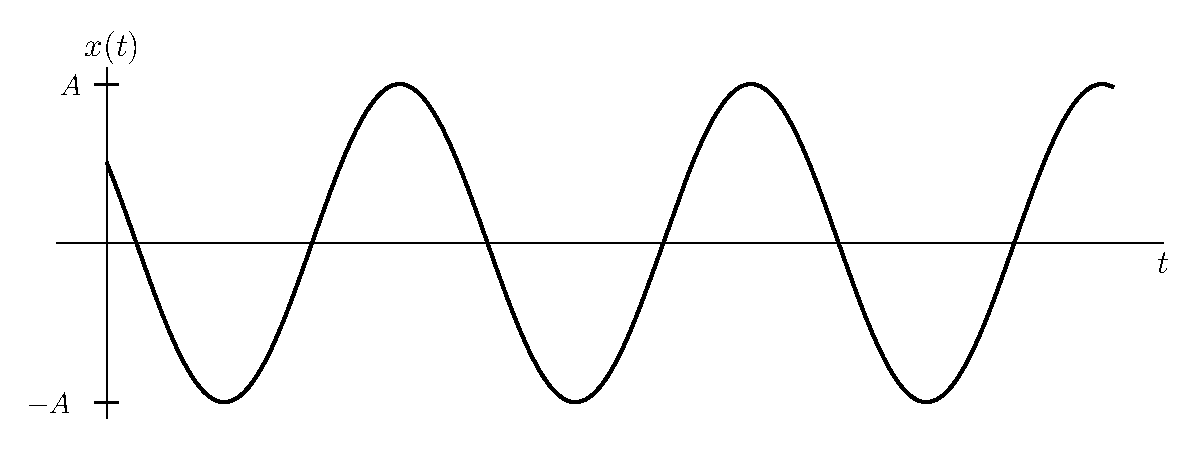
\includegraphics[scale=0.4]{fig_pos.pdf}
\end{center}

\end{topicbox}





\begin{topicbox}{Velocity and Acceleration}

\noindent We can calculate the velocity from the position,
\[
v(t) = \frac{dx}{dt} = -\omega A \sin (\omega t + \phi_0).
\]
\begin{center}
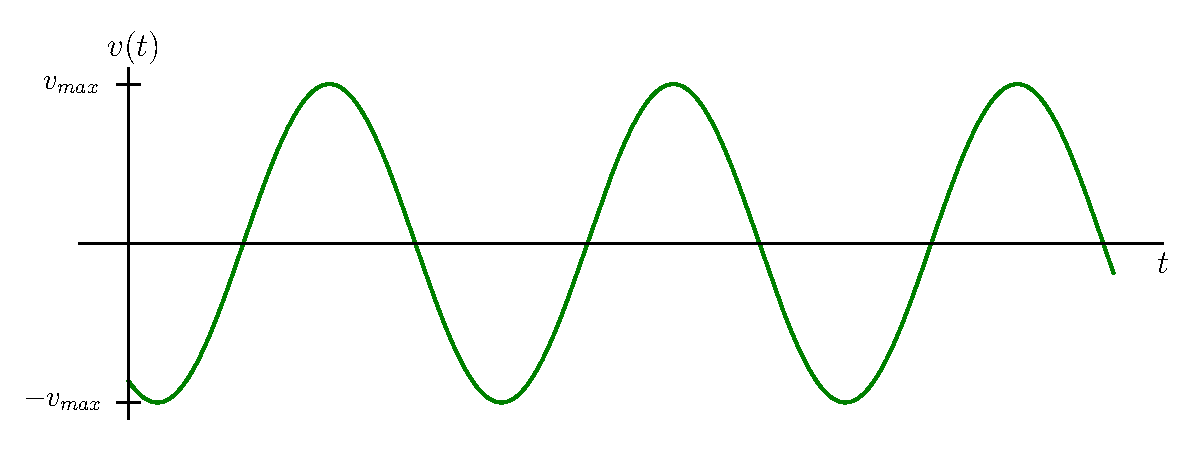
\includegraphics[scale=0.35]{fig_vel.pdf}
\end{center}
We can then calculate the acceleration from the velocity,
\[
a(t) = \frac{dv}{dt} = -\omega^2 A \cos(\omega t + \phi_0).
\]
Note that $a(t) = -\omega^2 x(t)$ as we expect.

\begin{center}
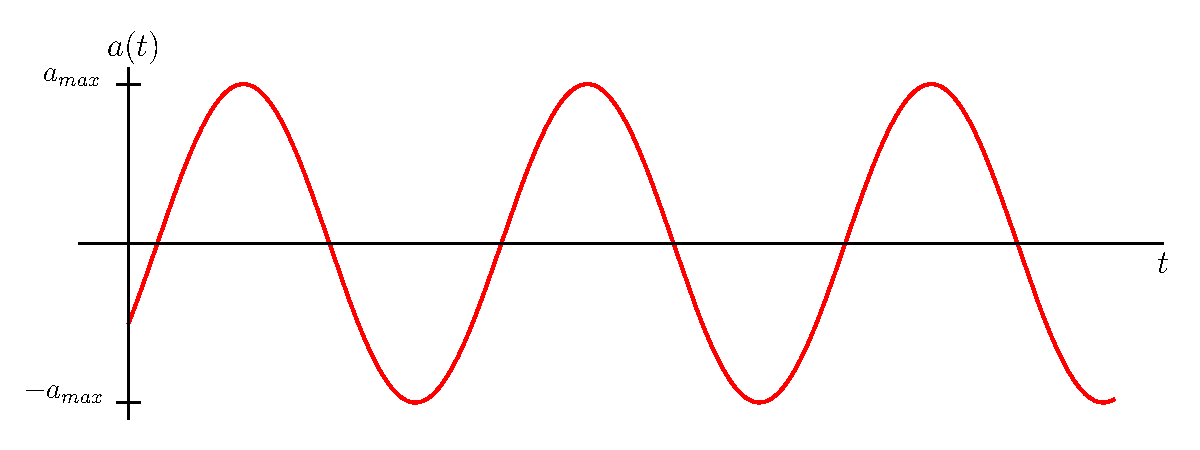
\includegraphics[scale=0.35]{fig_acc.pdf}
\end{center}


\end{topicbox}



\begin{topicbox}{Period and Frequency}

\noindent The time is takes to complete one full oscillation is called the \emph{period}, $T$.  The \emph{frequency} $f$ is the number of oscillations per second,
\[
f = \frac{1}{T},
\]
and is measured in hertz, 1 Hz = 1 s$^{-1}$.  The \emph{angular frequency} $\omega$ of the motion is related to the frequency and period by
\[
\omega = 2\pi f = \frac{2 \pi}{T}.
\]

\end{topicbox}


\begin{topicbox}{Energy in Simple Harmonic Motion}

\noindent The potential energy for an object in simple harmonic motion is just the elastic potential energy,
\[
U = \frac{1}{2} k x^2.
\]

If mechanical energy is conserved, 
\begin{eqbox}
E_\text{mech} = \frac{1}{2} mv^2 + \frac{1}{2}kx^2 = \frac{1}{2}mv_\text{max}^2 = \frac{1}{2}kA^2.
\end{eqbox}

\end{topicbox}


%\begin{topicbox}{The Small Angle Approximation}
%
%\noindent If an angle is small and measured in radians, then
%\begin{align*}
%\sin \theta & \approx \theta, \\
%\cos \theta & \approx 1, \\
%\tan \theta & \approx \theta.
%\end{align*}
%These approximations are good up to angles of around 10$^\circ$.
%
%\end{topicbox}

\begin{topicbox}{The Pendulum}

\noindent The pendulum is an oscillating system.  If the angular displacement of the bob remains small, then the small angle approximation can be used to write the differential equation describing the pendulum motion as
\[
\frac{d^2\theta}{dt^2} = -\omega^2 \theta,
\]
where $\omega = \sqrt{g/L}$ in this case.  This equation is similar to that for simple harmonic motion, so the pendulum also undergoes that type of motion:
\begin{eqbox}
\theta(t) = \theta_\text{max} \cos (\omega t + \phi_0).
\end{eqbox}

\end{topicbox}

\begin{topicbox}{Damped Oscillations}

\noindent If a system experiences a linear restoring force \emph{and} a drag force $F_\text{drag} = -bv$, where $b$ is called the damping parameter, then the differential equation that describes the system is
\[
\frac{d^2x}{dt^2} = \frac{b}{m} \frac{dx}{dt} + \frac{k}{m} x = 0A.
\]
This has the solution
\begin{eqbox}
x(t) = A e^{-bt/2m} \cos(\omega t + \phi_0),
\end{eqbox}
\noindent where the angular frequency is now
\[
\omega = sqrt{ \frac{k}{m} - \frac{b^2}{4m^2} }.
\]

The mechanical energy is not conserved in damped oscillations:
\[
E_\text{mech} = E_0 e^{-t/\tau},
\]
where $E_0 = \tfrac{1}{2}kA^2 = \tfrac{1}{2} mv_\text{max}^2$ is the initial mechanical energy of the system, and 
\[
\tau = \frac{m}{b}
\]
is called the \emph{time constant.}

\end{topicbox}



\end{multicols}





\makebanner{Mechanics}

\end{document}




